\section{The Fractional Linear Transformation}\label{Fractional_Section_Extended_Complex}

In this section a fractional linear transformation is derived from extending the stereographic projection between a $2$-sphere and the complex plane to Minkowskian space-time. The fixed points of this transformation are determined and found to be directly related to the null directions of a Lorentz transformation. Some examples of fractional linear transformations and their associated null directions are then given. 

\subsection{Stereographic Projection and the Extended Complex Plane}\label{Section_Stereographic_Extended_Complex}

First, a one to one mapping between the $2$-sphere, $\mathbb{S}^2$ and the extended complex plane $\hat{\mathbb{C}}$ is constructed. \textit{Stereographic projection} is the mapping of points on a sphere to points on a plane. In $\mathbb{R}^3$ with rectangular Cartesian coordinates $(x, y, z)$, consider the unit sphere with centre $(0,0,0)$, defined by

\begin{equation*}
\mathbb{S}^2 \subset \mathbb{R}^3 \text{ : } x^2 + y^2 + x^2 = 1.
\end{equation*}

\noindent The projection $P \rightarrow Q$ is a stereographic projection, see Fig.(\ref{Stereographic_Projecttion_Fig}). A relationship between $(X,Y,0)$ and $(x,y,z)$ is constructed as follows. $P$ is subdivided into the line segment $NQ$ in some ratio, $l:m$ say. 

\begin{figure}[h!]
\begin{center}
\caption{\textit{The projection from the unit $2$-sphere to the $x$,$y$-plane is called a Stereographic projection. The point $P$ on the shpere is mapped to the point $Q$ on the plane by translation along the line joining the points $N$ and $P$}}
\label{Stereographic_Projecttion_Fig}
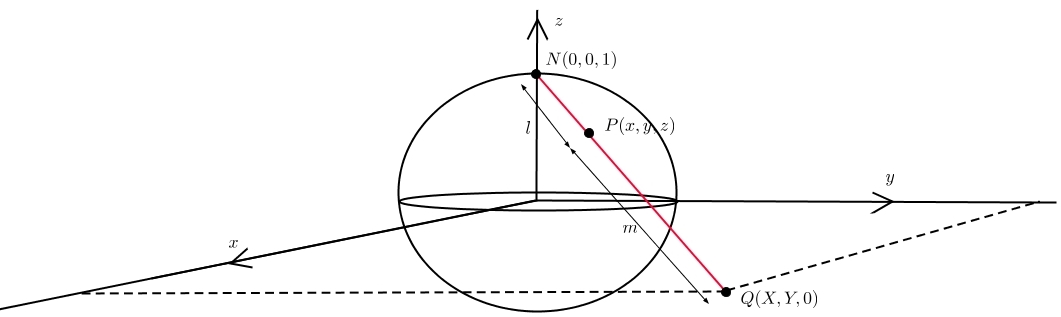
\includegraphics[scale=0.50]{figs/4_1.jpg}
\end{center}
\end{figure}

\noindent By coordinate geometry

\begin{eqnarray*}  
x = \frac{lX + mO}{l+m} = \frac{lX}{l+m}, \\
y = \frac{lY + mO}{l+m} = \frac{lY}{l+m}, \\
z = \frac{l.0+ m.1}{l+m} = \frac{m}{l+m}.
\end{eqnarray*}

\noindent Where O is the position of the origin. This implies that

\begin{eqnarray*}
1-z = \frac{l}{l+m}, \\
x = (1-z)X, \\
y = (1-z)Y.
\end{eqnarray*}

\noindent It is also known that $x^2+ y^2 +z^2 = 1$, so using this relation it is clear that

\begin{eqnarray*}
x^2 + y^2 = 1-z^2 = (1-z) (1+z), \\
(1-z)^2(X^2 +Y^2) = (1-z) (1+z).
\end{eqnarray*}

\noindent If the point $N$ is excluded, i.e. $z \neq 1$ then divide by $(1-z)^2$ to obtain

\begin{equation*} 
X^2 + Y^2 = \frac{1+z}{1-z},
\end{equation*}

\noindent and Rearrange to find

\begin{equation}\label{Ext_Complex_z_in_term_XY} 
z = \frac{X^2 + y^2 - 1}{X^2 + y^2 + 1}.
\end{equation}

Define $\zeta = X+ iY$ and rewrite Eqn.(\ref{Ext_Complex_z_in_term_XY}) to see that

\begin{equation*}
z = \frac{\zeta\bar{\zeta} - 1}{\zeta\bar{\zeta} + 1},
\end{equation*}

\noindent Which implies

\begin{equation*}
1- z = \frac{2}{\zeta\bar{\zeta} + 1}.
\end{equation*}

\noindent So relations for $(x,y,z) \in \mathbb{S}^2 \backslash \{N\}$ have been obtained in terms of $\zeta$, such that

\begin{align}\label{Ext_Complex_xy_interms_zeta}
x + iy & = \zeta (1-z) = \frac{2\zeta}{\zeta\bar{\zeta} + 1}, \\\label{Ext_Complex_z_interms_zeta}
z  & = \frac{\zeta\bar{\zeta} - 1}{\zeta\bar{\zeta} + 1}.
\end{align}

\noindent Hence the points on $\mathbb{S}^2 \backslash \{N\}$ are labelled by complex numbers $\zeta \in \mathbb{C}$. If a point $\zeta = \infty$, called the point at infinity of $\mathbb{C}$, is allowed then the following limits hold

\begin{eqnarray*}
x+ iy = \frac{2/\bar{\zeta}}{1 + 1/\zeta\bar{\zeta}} \rightarrow 0 \text{, as  } \zeta \rightarrow \infty, \\
z = \frac{1- 1/\zeta\bar{\zeta}}{1+ 1/\zeta\bar{\zeta}} \rightarrow 1 \text{, as  } \zeta \rightarrow \infty. 
\end{eqnarray*}

\noindent Then $N = (0,0,1)$ corresponds to $\zeta = \infty$. Thus in this way there is a one to one correspondence between the points of $\mathbb{S}^2$ and the points of the \textit{extended complex plane} $\hat{\mathbb{C}} = \mathbb{C} \cup {\infty}$, which is the usual complex plane with the point at infinity added. Since $\mathbb{S}^2$ has finite surface area, and is therefore called a \textit{compact manifold}, the identification of the points of $\hat{\mathbb{C}}$ with the points of $\mathbb{S}^2$ is called the \textit{compactification} of $\hat{\mathbb{C}}$.

The pair $(\zeta, \bar{\zeta})$ are called the \textit{stereographic coordinates} on $\mathbb{S}^2 \backslash \{N\}$. How are they related to the polar angles $\theta$ and $\phi$? To investigate this write the usual spherical polar coordinates in terms of $\zeta$. First it is known that

\begin{align*}
x & = \sin{\theta}\cos{\phi}, \\
y & = \sin{\theta}\sin{\phi}, \\
z & = \cos{\theta}.
\end{align*}

\noindent So by Eqn.(\ref{Ext_Complex_z_interms_zeta}) it is clear that

\begin{gather*}
z = \cos{\theta} = \frac{\zeta\bar{\zeta} - 1}{\zeta\bar{\zeta} + 1} \\
\zeta\bar{\zeta}\cos{\theta} + \cos{\theta} = \zeta\bar{\zeta} - 1\\
\zeta\bar{\zeta} = \frac{1 + \cos{\theta}}{1 - \cos{\theta}} = \frac{2\cos^2{\left(\theta/2\right)}}{2\sin^2{\left(\theta/2\right)}} \\
\zeta\bar{\zeta} = \cot^2{\left(\theta/2\right)}.
\end{gather*}

\noindent Now use Eqn.(\ref{Ext_Complex_xy_interms_zeta}) to obtain

\begin{gather*}
\sin{\theta}(\cos{\phi} +i \sin{\phi}) = \frac{2\zeta}{\cot^2{\left(\theta/2\right)} + 1 }, \\
2\sin{\left(\theta/2\right)}\cos{\left(\theta/2\right)}e^{i\phi} = 2\zeta \sin^2{\left(\theta/2\right)}, \\
\zeta = e^{i\phi}\cot{\left(\theta/2\right)}. 
\end{gather*}

\noindent This makes sense as if $\zeta = \infty$ then $\theta = 0$ as one would expect. In summary the following coordinate transformations have been constructed

\begin{align}
\vec{n} = (x, y, z) & = (\sin{\theta}\cos{\phi}, \sin{\theta}\sin{\phi}, \cos{\theta}), \\ \label{Ext_Complex_Vec_n}
&
\begin{Huge}
                     = \left( \frac{\bar{\zeta} + \zeta}{\bar{\zeta}\zeta + 1}  ,i\frac{\bar{\zeta} - \zeta}{\bar{\zeta}\zeta + 1}, \frac{\bar{\zeta}\zeta - 1}{\bar{\zeta}\zeta + 1}  \right),
\end{Huge}
\end{align}

\noindent where here $\vec{n}$ is a unit vector in $\mathbb{R}^3$ such that $\vec{n} \cdot \vec{n} = 1$.

\subsection{Extension to Minkowskian Sapce-Time}\label{Fractional_Section_Extension_to_Minkowskian}

These results are now extended to Minkowskian space-time to derive an expression for the fractional Linear transformation. Let $\vec{x} = (x,y,z,t)$ be a point on the future null cone with origin $(0,0,0,0)$. Denote the future null cone as $N^{+}$, so that 

\begin{equation*}
N^+ : x^2 + y^2 + z^2 - t^2 = 0 \text{,  for  } t>0,
\end{equation*}

\noindent as all the vectors in the null cone have a Lorentz quadratic form equal to zero by definition. The intersection with the space-like hypersurface $t = \text{const}>0$ is a 2-sphere denoted by 

\begin{equation}\label{Ext_Complex_2Sphere_Definition}
\mathbb{S}^2 (t) : x^2 + y^2 + z^2 = t^2 = \text{const}, 
\end{equation}

\noindent see Fig.(\ref{Ext_Complex_Intersection_Cone_Plane_Fig}). There is a generator of $N^+$ passing through each point of $\mathbb{S}^2 (t)$, they are the null geodesics tangent to $N^+$ and passing through the point $(0,0,0,0)$. Hence the points of $\mathbb{S}^2 (t)$, denoted by $(\theta,\phi)$ or $\zeta$, label the \textit{generators} of $N^{+}$.

\begin{figure}[h!]
\begin{center}
\caption{\textit{Future null cone of Minkowskian space-time. Shown in red is the intersection between the future null cone and the hyperplane $t=\text{const}$. This surface is the sphere in three dimensions from which a stereographic projection was derived earlier.}}
\label{Ext_Complex_Intersection_Cone_Plane_Fig}
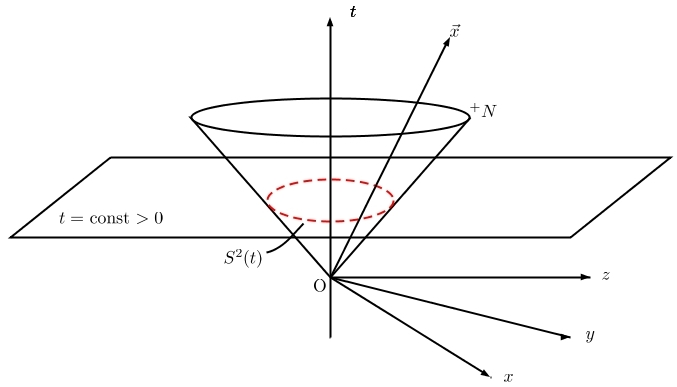
\includegraphics[scale=0.6]{figs/4_5.jpg}
\end{center}
\end{figure}

For every generator and any $t>0$ it is clear that

\begin{equation*}
\left(\frac{x}{t}\right)^2 +\left(\frac{y}{t}\right)^2 +\left(\frac{z}{t}\right)^2 = 1.
\end{equation*}

\noindent This is just the definition of a $2$-sphere, as in Eqn.(\ref{Ext_Complex_2Sphere_Definition}), normalised with respect to a constant $t$. Hence we can write $\vec{x}$ in terms of the coordinate transformation of (\ref{Ext_Complex_Vec_n})

\begin{align}\nonumber
\vec{x} & = t(\sin{\theta}\cos{\phi}, \sin{\theta}\sin{\phi}, \cos{\theta}, 1), \\\label{Ext_Complex_vec_x_relations}
        & = t
\begin{Huge}
\left( \frac{\bar{\zeta} + \zeta}{\bar{\zeta}\zeta + 1}  ,i\frac{\bar{\zeta} - \zeta}{\bar{\zeta}\zeta + 1}, \frac{\bar{\zeta}\zeta - 1}{\bar{\zeta}\zeta + 1},1  \right).
\end{Huge}
\end{align}

\noindent Where a $4^{\text{th}}$ component is included as $\vec{x}$ is an element of Minkowskian space-time. Thus the direction of $\vec{x}$ is determined explicitly by $(\theta,\phi)$ or $\zeta$ as $\vec{x}$ has the same form as the unit vector of Eqn.(\ref{Ext_Complex_Vec_n}). Note that all possible directions of $\vec{x}$ on $N^{+}$ are covered if $\zeta \in \hat{\mathbb{C}}$. Now the Lorentz transformation $\vec{x} \rightarrow \vec{x}'$ is investigated, it takes the form  

\begin{equation*}
\vec{x} \rightarrow \vec{x}' = t'\left( \frac{\bar{\zeta'} + \zeta'}{\bar{\zeta'}\zeta' + 1}  ,i\frac{\bar{\zeta'} - \zeta'}{\bar{\zeta'}\zeta' + 1}, \frac{\bar{\zeta'}\zeta' - 1}{\bar{\zeta'}\zeta' + 1},1  \right).
\end{equation*}

\noindent The null direction $\zeta$ is transformed to the null direction $\zeta'$, where the relation between them must be determined. Construct the matrix $A(\vec{x})$ as in Eqn.(\ref{Special_Matrices_A_first}),

\begin{equation*}
A(\vec{x}) = 
\left(
\begin{array}{ccc}
\frac{2t}{\zeta\bar{\zeta}+1} & & \frac{2t\zeta}{\zeta\bar{\zeta}+1} \\
 & & \\
\frac{2t\bar{\zeta}}{\zeta\bar{\zeta}+1} & & \frac{2t\zeta\bar{\zeta}}{\zeta\bar{\zeta}+1} \\
\end{array}
\right)
=
c_0\left(
\begin{array}{cc}
1           & \zeta \\ 
\bar{\zeta} & \bar{\zeta}\zeta \\ 
\end{array}
\right),
\end{equation*}

\noindent where $c_0 = 2t/(\zeta\bar{\zeta}+1) \in \mathbb{R}^2$. Note that as $\vec{x}$ is a null vector $\det{(A(\vec{x}))} = 0$. Thus the transformed matrix $A(\vec{x}')$ is given similarly as

\begin{equation*}
A(\vec{x}') = 
{c_0}'\left(
\begin{array}{cc}
1           & \zeta' \\ 
\bar{\zeta'} & \bar{\zeta'}\zeta' \\ 
\end{array}
\right).
\end{equation*}

\noindent Now, as in the examples in section (\ref{Special_Linear_Matrices_of_Lorentz}) we determine the special linear matrix $U$ such that

\begin{equation}\label{Ext_Complex_UAU}
A(\vec{x}') = U A(\vec{x}) U^{\dagger}
\end{equation}

\noindent As before, this matrix equation is written component wise as

\begin{equation*}
{c_0}'\left(
\begin{array}{cc}
1           & \zeta' \\ 
\bar{\zeta'} & \bar{\zeta'}\zeta' \\ 
\end{array}
\right)
=
\left(
\begin{array}{cc}
\alpha & \beta \\
\gamma & \delta \\
\end{array}
\right)
{c_0}\left(
\begin{array}{cc}
1           & \zeta \\ 
\bar{\zeta} & \bar{\zeta}\zeta \\ 
\end{array}
\right)
\left(
\begin{array}{cc}
\bar{\alpha} & \bar{\beta} \\
\bar{\gamma} & \bar{\delta} \\
\end{array}
\right).
\end{equation*}

\noindent Then three separate relations between $\zeta$ and $\zeta'$ are obtained

\begin{align}\label{Ext_Complex_zeta_trans_1} 
{c_0}' & = c_0 (\alpha \bar{\alpha} + \alpha \bar{\beta} \zeta + \bar{\alpha} \beta \bar{\zeta} + \beta \bar{\beta} \zeta \bar{\zeta}), \\\label{Ext_Complex_zeta_trans_2} 
{c_0}'\zeta' & = c_0 (\alpha \bar{\gamma} + \alpha \bar{\delta} \zeta + \bar{\gamma} \beta \bar{\zeta} + \beta \bar{\delta} \zeta \bar{\zeta}), \\\label{Ext_Complex_zeta_trans_3} 
{c_0}'\zeta'\bar{\zeta'} & = c_0 (\gamma \bar{\gamma} + \gamma \bar{\delta} \zeta + \bar{\gamma} \delta \bar{\zeta} + \delta \bar{\delta} \zeta \bar{\zeta}). 
\end{align} 

\noindent Using Eqns.(\ref{Ext_Complex_zeta_trans_1}) and (\ref{Ext_Complex_zeta_trans_2}) and factorising to obtain

\begin{equation*}
\zeta' = \frac{{c_0}'\zeta'}{{c_0}'} = \frac{\alpha(\bar{\gamma} + \bar{\delta}\zeta) + \beta \bar{\zeta}(\bar{\gamma} + \bar{\delta}\zeta)}{\alpha(\bar{\alpha} + \bar{\beta}\zeta) + \beta \bar{\zeta}(\bar{\alpha} + \bar{\beta}\zeta)} \\
\end{equation*}

\noindent Thus 

\begin{equation}\label{Extended_Complex_Fractional_Linear_Transformation}
\zeta' = \frac{(\bar{\gamma} + \bar{\delta}\zeta)}{(\bar{\alpha} + \bar{\beta}\zeta)},
\end{equation}

\noindent with $\alpha\delta - \beta\gamma = 1$ as before. This is a \textit{fractional linear transformation} of the extended complex plane $\hat{\mathbb{C}}$. There is a one to one correspondence here between proper, orthochronous Lorentz transformations and fractional linear transformations of the extended complex plane. This is because the matrices $\pm U$ both satisfy Eqn.(\ref{Ext_Complex_UAU}) as in the previous section, but now both matrices give the same transformation as the signs will cancel in the fractional transformation.

\subsection{Fixed points and Their Associated Null Directions}

A given Lorentz transformation is equivalent to known $\alpha$, $\beta$ , $\gamma$ and $\delta$ parameters module a sign and therefore gives an explicit fractional linear transformation. For a given Lorentz transformation a \textit{fixed point} of the corresponding fractional linear transformation corresponds to an invariant null direction. The fixed points $\zeta$ satisfy the relation $\zeta' = \zeta$. Thus from Eq.(\ref{Extended_Complex_Fractional_Linear_Transformation})

\begin{gather}\nonumber
\zeta' = \frac{(\bar{\gamma} + \bar{\delta}\zeta)}{(\bar{\alpha} + \bar{\beta}\zeta)} = \zeta, \\\label{Ext_Complex_fixed_point}
\bar{\beta}\zeta^2 + (\bar{\alpha}- \bar{\delta})\zeta - \bar{\gamma} = 0. 
\end{gather}

\noindent Clearly this is a quadratic equation over the field $\mathbb{C}$, thus it has two roots in general. The non-singular case is when these roots do not coincide, hence a Lorentz transformation does indeed leave two null directions invariant in general.  If Eqn.(\ref{Ext_Complex_fixed_point}) has only one root then the corresponding Lorentz transformation leaves one null direction invariant, this is the singular case.

Consider Eqn.(\ref{Ext_Complex_fixed_point}) again. Divide by $\zeta^2$ to obtain

\begin{equation*}
\bar{\beta} + (\bar{\alpha}- \bar{\delta})\zeta^{-1} - \bar{\gamma}\zeta^{-2} = 0.
\end{equation*}

\noindent Hence $\zeta = \infty$ is a solution of this equation if $\beta = 0$. If $\zeta = \infty$ then $\vec{x}$ is given by $\vec{x} = t(0,0,1,1)$ by Eqn.(\ref{Ext_Complex_vec_x_relations}). Thus it is clear that this corresponds to the null direction $z=t$. Compare this to Example 3, Section (\ref{Special_Linear_Matrices_Example_3}). Here $\beta$ is zero AND the null direction is $z=t$ as expected. If $\zeta = 0$ is a solution to Eqn.(\ref{Ext_Complex_fixed_point}) it is required that $\gamma = 0$, thus $\vec{x} = (0,0,-1,1)$. So it is predicted that a Lorentz transformation with a special linear matrix of the form

\begin{equation*}   
U = 
\left(
\begin{array}{cc}
\alpha & \beta \\
0 & \delta \\
\end{array}
\right),
\end{equation*}   

\noindent will leave the $z=-t$ null direction invariant. The example in section (\ref{Ext_Complex_Ex_end}) illustrates a case where the null direction is found to be $x=\pm t$, due to the form of the matrix $U$. The choice of the components of the matrix $A$ in Eqn.(\ref{Special_Matrices_A_first}) determine which direction is the null direction. The initial choice of $A$ gives special significance to the $z$ component, this of course is arbitrary. In Appendix (\ref{Appendix_Special_Significance_x}), the example in Section (\ref{Special_Linear_Matrices_Example_3}) is repeated for the case when special significance is given to $x$. 

\subsection{Example: Standard Lorentz Transformation}\label{Ext_Complex_Ex_end}

Continuing on from Example 2, section (\ref{Special_Linear_Matrices_Example_2}), where $\alpha$, $\beta$, $\gamma$ and $\delta$ were determined. $\zeta'$ can now be expressed as a fractional linear transformation by Eqn.(\ref{Extended_Complex_Fractional_Linear_Transformation})

\begin{equation*} 
\zeta' = \frac{-\sqrt{\gamma_0 - 1} + \sqrt{\gamma_0 + 1}\zeta}{\sqrt{\gamma_0 + 1} - \sqrt{\gamma_0 - 1}\zeta}.
\end{equation*}

\noindent If the condition $\zeta' = \zeta$ is imposed then

\begin{gather*}
\sqrt{\gamma_0 - 1}(\zeta^2 - 1) = 0, \\
\zeta = \pm 1.
\end{gather*}

In the $\zeta = +1$ case, $\vec{x} = t(1,0,0,1)$ and the invariant direction is $x=t$. Similarly in the $\zeta = -1$ case $\vec{x} = t(-1,0,0,1)$ and the invariant direction is $x = - t$. 



   












